%!TEX root = paper.tex

\subsection{Abstract Specs \& Concretization}
	\todo{.75 page}
	

\begin{figure}
	\centering
	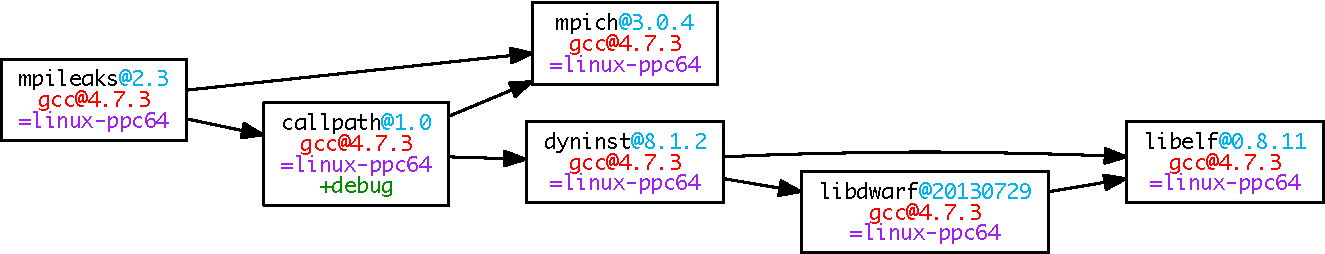
\includegraphics[width=\columnwidth]{specs/mpileaks-concrete.pdf}
	\caption{
		Concretized version of specs from Figure~\ref{fig:specs-mpileaks}.
		\label{fig:specs-mpileaks-concrete}
	}
\end{figure}



{\bf Dependencies.}
Lines 6 and 7 in the table show the key feature that enables Spack's flexibility.
The user can specify all of the above information not only for the package being
installed, but also for its {\it dependencies}.  To do this, the user needs only supply 
\verb|^| and the dependency's name.  If we need to build a new version with a specific
version of {\tt mvapich2}, we can simply add, e.g., \verb|^mvapich2@1.9|
to the spec, and it will build with that MPI version instead of the default.
This can also be done for multiple libraries in the same spec (line 7).  




Before it builds a package, Spack ensures the following conditions:
\newline

\begin{tabular}{l}
(1) All dependencies are present in the DAG. \\
(2) Parameters are set on all packages in the DAG. \\
\end{tabular}\newline

\noindent
The install process then constructs a package object for each node in the spec DAG
and traverses the DAG in a bottom-up fashion.  At each node, it invokes the package's
{\tt install()} method, using a sub-DAG rooted at the package to be installed as the {\tt spec}
parameter to {\tt install()}. Package maintainers are responsible for examining the spec's
configuration and adjusting the build if necessary.


In our experience, much complexity in build scripts arises from the need for the script to
query the environment and determine how to build.  In spack, build scripts are free from this 
concern, because the package author is guaranteed that a package's build spec is concrete
by the time {\tt install()} is called. There is thus no need to perform complicated state checks,
just to query the spec for its configuration.


